\documentclass[]{article}
\usepackage{lmodern}
\usepackage{amssymb,amsmath}
\usepackage{ifxetex,ifluatex}
\usepackage{fixltx2e} % provides \textsubscript
\ifnum 0\ifxetex 1\fi\ifluatex 1\fi=0 % if pdftex
  \usepackage[T1]{fontenc}
  \usepackage[utf8]{inputenc}
\else % if luatex or xelatex
  \ifxetex
    \usepackage{mathspec}
  \else
    \usepackage{fontspec}
  \fi
  \defaultfontfeatures{Ligatures=TeX,Scale=MatchLowercase}
\fi
% use upquote if available, for straight quotes in verbatim environments
\IfFileExists{upquote.sty}{\usepackage{upquote}}{}
% use microtype if available
\IfFileExists{microtype.sty}{%
\usepackage[]{microtype}
\UseMicrotypeSet[protrusion]{basicmath} % disable protrusion for tt fonts
}{}
\PassOptionsToPackage{hyphens}{url} % url is loaded by hyperref
\usepackage[unicode=true]{hyperref}
\hypersetup{
            pdfborder={0 0 0},
            breaklinks=true}
\urlstyle{same}  % don't use monospace font for urls
\usepackage{graphicx,grffile}
\makeatletter
\def\maxwidth{\ifdim\Gin@nat@width>\linewidth\linewidth\else\Gin@nat@width\fi}
\def\maxheight{\ifdim\Gin@nat@height>\textheight\textheight\else\Gin@nat@height\fi}
\makeatother
% Scale images if necessary, so that they will not overflow the page
% margins by default, and it is still possible to overwrite the defaults
% using explicit options in \includegraphics[width, height, ...]{}
\setkeys{Gin}{width=\maxwidth,height=\maxheight,keepaspectratio}
\IfFileExists{parskip.sty}{%
\usepackage{parskip}
}{% else
\setlength{\parindent}{0pt}
\setlength{\parskip}{6pt plus 2pt minus 1pt}
}
\setlength{\emergencystretch}{3em}  % prevent overfull lines
\providecommand{\tightlist}{%
  \setlength{\itemsep}{0pt}\setlength{\parskip}{0pt}}
\setcounter{secnumdepth}{0}
% Redefines (sub)paragraphs to behave more like sections
\ifx\paragraph\undefined\else
\let\oldparagraph\paragraph
\renewcommand{\paragraph}[1]{\oldparagraph{#1}\mbox{}}
\fi
\ifx\subparagraph\undefined\else
\let\oldsubparagraph\subparagraph
\renewcommand{\subparagraph}[1]{\oldsubparagraph{#1}\mbox{}}
\fi

% set default figure placement to htbp
\makeatletter
\def\fps@figure{htbp}
\makeatother


\date{}

\begin{document}

\protect\hypertarget{page2}{}{}\textbf{Réplique de la mission InSIGHT}

\begin{quote}
L'étude proposée porte sur la réplique terrestre\textsuperscript{1} du
système InSIGHT (\textbf{In}terior exploration using \textbf{S}eismic
\textbf{I}nvestigations, \textbf{G}eodesy and \textbf{H}eat
\textbf{T}ransport), projet du CNES (Centre National d'Études Spatiales)
qui a pour but de déployer une station d'étude de la structure interne
de la planète Mars.

La station de mesures doit effectuer une campagne de mesures de
l'activité sismique afin d'établir des informations sur l'épaisseur de
la croûte martienne, de ses manteaux et des zones de subduction, voire
des impacts des météorites.

Le support technologique de la mission est un atterrisseur similaire à
celui de la mission Phoenix qui a été utilisé avec succès en 2007 pour
étudier le sol glacé près du pôle nord de Mars.
\end{quote}


\includegraphics[width=3.08819in,height=2.31667in]{media/image1.jpeg}

\textbf{Figure 1} -- Atterrisseur du projet InSIGHT

\begin{quote}
L'atterrisseur InSIGHT (\textbf{figure 1}) emportera quatre
sous-systèmes d'instrumentation à la surface de

Mars afin d'analyser en détail pour la première fois les "statistiques
vitales" de la planète :
\end{quote}

\begin{itemize}
\item
  \begin{quote}
  son pouls, activité interne, mesuré par l'instrument SEIS ;
  \end{quote}
\item
  \begin{quote}
  sa température mesurée par l'instrument HP³ ;
  \end{quote}
\item
  \begin{quote}
  ses réflexes mesurés par l'instrument RISE.
  \end{quote}
\end{itemize}

\begin{quote}
Ensemble, les données fourniront des indices essentiels sur l'évolution,
non seulement de la planète Mars, mais aussi de toutes les planètes
telluriques.

\emph{Sous-systèmes d'instrumentation de l'atterrisseur}
\end{quote}

\begin{itemize}
\item
  \begin{quote}
  \textbf{SEIS} : sismomètre qui fera des mesures précises des
  tremblements et autres activités internes de Mars pour mieux
  comprendre l'histoire et la structure de la planète ;
  \end{quote}
\item
  \begin{quote}
  \textbf{HP³} : cet instrument va s'enfoncer, à cinq mètres de
  profondeur sous la surface de Mars, pour connaître la quantité de
  chaleur venant de l'intérieur de Mars et pour révéler l'histoire
  thermique de la planète ;
  \end{quote}
\item
  \begin{quote}
  \textbf{RISE} : il s'agit d'une expérience qui mesurera avec précision
  le décalage Doppler et le parcours des communications radio entre
  l'atterrisseur InSIGHT et la Terre pour déterminer la distribution des
  structures internes de la planète rouge ;
  \end{quote}
\item
  \begin{quote}
  \textbf{Camera} : montée sur le bras de l'atterrisseur, elle servira à
  prendre des images en noir et blanc des instruments sur le corps de
  l'atterrisseur ainsi qu'une vue en 3D pour aider les ingénieurs et les
  scientifiques à guider le déploiement des instruments au sol.
  \end{quote}
\end{itemize}

\begin{enumerate}
\def\labelenumi{\arabic{enumi}.}
\item
  Utilisée sur Terre pour validation des différents sous-systèmes.
\end{enumerate}

\protect\hypertarget{page3}{}{}\textbf{Seul le sous-système SEIS}
(\textbf{figure 2}) \textbf{sera l'objet de l'étude proposée}. Il est
basé sur un instrument hybride composé \textbf{:}

\begin{itemize}
\item
  \begin{quote}
  d'un système de déploiement (DPL) ;
  \end{quote}
\item
  \begin{quote}
  d'une sphère comportant trois capteurs sismiques à très larges bandes
  et leurs capteurs de température. La sphère dispose d'un système de
  référencement de ses pieds (\textbf{figure 3}). Sa masse est d'environ
  3 kg et sa consommation électrique varie autour de 1W.
  \end{quote}
\item
  \begin{quote}
  d'une boîte électronique d'acquisition dont la structure est donnée
  par le diagramme de définition des blocs de la \textbf{figure 4}.
  \end{quote}
\end{itemize}

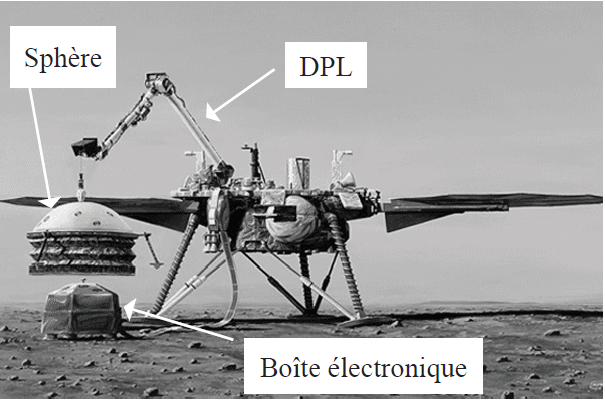
\includegraphics[width=6.63599in,height=2.65116in]{media/image2.png}


\includegraphics[width=6.10465in,height=3.95886in]{media/image3.png}

\textbf{Figure 4} -- Diagramme de définition des blocs

La \textbf{figure 5} (page 3) présente le diagramme des cas
d'utilisation du système de positionnement DPL et du module SEIS et la
\textbf{figure 6} (page 3) le diagramme partiel des exigences concernant
le système de déploiement DPL et le module SEIS.\textbf{\\
}


\includegraphics[width=6.20930in,height=3.95625in]{media/image4.png}


\includegraphics[width=6.43591in,height=5.29070in]{media/image5.png}

\textbf{Figure 6} -- Diagramme partiel des exigences

\protect\hypertarget{page5}{}{}
\includegraphics[width=6.58367in,height=3.08333in]{media/image6.png}


\includegraphics[width=3.38542in,height=1.95139in]{media/image7.jpeg}

Le bras de déploiement est constitué de :

\emph{Bâti : 0}

\begin{quote}
Le repère
\(R_{0}({\overrightarrow{x}}_{0},{\overrightarrow{y}}_{0},{\overrightarrow{z}}_{0})\ \ \)
est lié au bâti fixe 0.
\end{quote}

\emph{Bras : 1}

\begin{quote}
Repère lié
\(R_{1}({O,\overrightarrow{x}}_{1},{\overrightarrow{y}}_{1},{\overrightarrow{z}}_{1})\ \ \)

Mouvement (1/0) : rotation autour de
\(\left( O{\overrightarrow{z}}_{0} \right)\)

Position (1/0) repérée par :
\(\theta_{1} = (\ {\overrightarrow{x}}_{0},\ {\overrightarrow{x}}_{1}) = ({\overrightarrow{y}}_{0},{\overrightarrow{y}}_{1})\)

Centre d'inertie G\textsubscript{1} tel que
\(\overrightarrow{OG_{1}} = \ \frac{L}{2}\ {\overrightarrow{x}}_{1}\ \)avec
\(\overrightarrow{\text{OQ}} = \ \ {L\overrightarrow{x}}_{1}\)

Masse \emph{m}\textsubscript{1} = 352 \emph{g} ; \emph{L} = 0,5\emph{m}.
\end{quote}

La \textbf{figure 8} présente le modèle volumique du bras 1. Les plans
\(\left( G_{1},\ {\overrightarrow{x}}_{1},\ {\overrightarrow{y}}_{1} \right)\ \text{et}\ \left( G_{1},\ {\overrightarrow{y}}_{1},\ {\overrightarrow{z}}_{1}\  \right)\)
sont des plans de symétrie matérielle du bras 1.

Le mouvement de 1 par rapport à 0 est commandé par un actionneur
\emph{M}\textsubscript{01}, constitué d'un moteur pas à pas et d'un
réducteur de vitesse à couronne dentée flexible de rapport de
transmission λ = 82, d'encombrement et de masse très faibles en regard
des autres solides, logés à l'intérieur de la liaison (0/1).

\emph{Avant- bras : 2}

\begin{quote}
Repère lié
\(R_{2}({Q,\overrightarrow{x}}_{2},{\overrightarrow{y}}_{2},{\overrightarrow{z}}_{2})\ \ \)

Mouvement (2/0) : rotation autour de
\(\left( Q{\overrightarrow{z}}_{1} \right)\)

Position (2/0) repérée par :
\(\theta_{2} = (\ {\overrightarrow{x}}_{1},\ {\overrightarrow{x}}_{2}) = ({\overrightarrow{y}}_{1},{\overrightarrow{y}}_{2})\)

Masse \emph{m}\textsubscript{2} = 352 \emph{g }

Centre d'inertie G\textsubscript{2} tel que
\(\overrightarrow{QG_{2}} = \ \frac{L}{2}\ {\overrightarrow{x}}_{2}\ \)(L=0,5m)
avec \(\overrightarrow{\text{QP}} = \ \ {L\overrightarrow{x}}_{2}\) (le
bras 1 et l'avant bras 2 ont la même longueur)

L'extrémité en \emph{P} est équipée d'une pince de masse négligeable qui
saisit la sphère SEIS.

On note \emph{K\textsubscript{O}}\textsubscript{2} le moment d'inertie
de l'avant-bras 2 par rapport à l'axe
\(\left( O{\overrightarrow{z}}_{0} \right)\) dans la position la plus
défavorable.
\end{quote}

\protect\hypertarget{page6}{}{}

\begin{quote}
Le mouvement de 2 par rapport à 1 est commandé par un actionneur
\emph{M}\textsubscript{12}, constitué d'un moteur pas à pas et d'un
réducteur de vitesse à couronne dentée flexible de rapport de
transmission λ = 82, d'encombrement et de masse très faibles en regard
des autres solides, logés à l'intérieur de la liaison (1/2).

\emph{Sphère du SEIS : S}

On considère que l'amplitude du mouvement (S/2) est très faible.

Position (S/0) repérée par :
\(\overrightarrow{\text{OP}} = X_{P}(t){\overrightarrow{x}}_{0} + Y_{P}(t){\overrightarrow{y}}_{0}\ \)

Masse \emph{m\textsubscript{s}} = 1, 2 \emph{kg} considérée comme
ponctuelle en son centre d'inertie \emph{G\textsubscript{S}} par rapport
aux autres mouvements. \emph{G\textsubscript{S}} est tel que
\(\overrightarrow{PG_{s}} = - R{\overrightarrow{y}}_{0}\ \) (\emph{R}
est une constante positive).

On note \emph{K\textsubscript{OS}} le moment d'inertie de la sphère S
par rapport à l'axe \(\left( O{\overrightarrow{z}}_{0} \right)\) dans la
position \emph{θ}\textsubscript{1} = \emph{θ}\textsubscript{2} = 0 .

\textbf{Partie I - Validation des capacités de positionnement du système
de déploiement}

\emph{\textbf{Objectif} : vérifier l'exigence 002 « Position de la pince
» afin que le point de préhension P du système de déploiement DPL puisse
être défini à partir de deux coordonnées articulaires.}

\textbf{Q1} \emph{Etablir la relation vectorielle entre
X\textsubscript{p}, Y\textsubscript{p}, L et}
\({\overrightarrow{x}}_{0},\ \ {\overrightarrow{y}}_{0},\ {\overrightarrow{x}}_{1},\ {\overrightarrow{y}}_{1}\)\emph{.}

\textbf{Q2} \emph{Projeter la relation précédente selon}
\({\overrightarrow{x}}_{0},\ \ {\overrightarrow{y}}_{0}\)\emph{, puis
donner les deux équations scalaires correspondantes.}

\textbf{Q3} \emph{Exprimer θ\textsubscript{1} et θ\textsubscript{2} en
fonction de X\textsubscript{p}, Y\textsubscript{p}, L. Conclure quand au
respect de l'exigence 002}

\textbf{Partie II - Validation du non-dépassement de la vitesse de la
sphère SEIS}

\emph{\textbf{Objectif} : valider l'exigence 003 « Vitesse de la pince »
quand la sphère SEIS se déplace en translation afin de conserver
toujours la même orientation.}

\emph{Notation} :

\({\overrightarrow{V}}_{M,S/R}\text{\ \ }\)est le vecteur vitesse du
point \emph{M} appartenant au solide \emph{S} par rapport à \emph{R}.

\textbf{Q4} \emph{Déterminer l'expression de la vitesse du point P,
appartenant à l'avant bras 2 par rapport à R\textsubscript{0} en
fonction de θ\textsubscript{1}, θ\textsubscript{2} et L.}

\textbf{Q5} \emph{Déterminer la valeur maximale du taux de rotation}
\(\left\| {\overrightarrow{\Omega}}_{1/0} \right\|\ \) \emph{pour que
l'avant-bras 2 suive un mouvement de translation circulaire par rapport
à R\textsubscript{0} en respectant l'exigence 003 « Vitesse de la pince
».}
\end{quote}

\protect\hypertarget{page7}{}{}\textbf{Partie III - Validation de la
capacité statique du système de déploiement}

\begin{quote}
\emph{\textbf{Objectif} : déterminer le couple statique du
moto-réducteur M}01 \emph{qui permet l'équilibre du système de
déploiement.}

\emph{Spécification}

\(\overrightarrow{g}\  = \  - g{\overrightarrow{y}}_{0}\ \) est
l'accélération du champ de pesanteur terrestre\textsuperscript{2} avec
\emph{g} = 9,81 m·s\textsuperscript{--2}.

\textbf{Q6.} Exprimer puis calculer le couple statique, noté \emph{C}01,
que doit exercer le moto-réducteur \emph{M}01 dans la position du
système de déploiement la plus défavorable. Préciser clairement le
système isolé ainsi que le principe/théorème utilisé.

\textbf{Q7.} En déduire la valeur minimale du couple de maintien, noté
\emph{C}m1min, dont doit disposer le moteur pas à pas.

\emph{\textsuperscript{2}Rappel} : le système est une réplique
terrestre.
\end{quote}

\textbf{Partie IV - Validation des capacités dynamiques du système de
déploiement}

\begin{quote}
\emph{\textbf{Objectif} : déterminer le couple du moto-réducteur M}01
\emph{qui permet la manipulation de la sphère SEIS par le système de
déploiement.}

La \textbf{figure 7} (page 5) présente la schématisation du bras de
déploiement, noté Σ = \{1, 2, \emph{S}\}.
\end{quote}

\textbf{Q8.} Justifier que la matrice d'inertie du bras 1, en son centre
d'inertie G\textsubscript{1}, est de la forme :

\[J(G_{1},1) = \begin{bmatrix}
I_{1} & 0 & 0 \\
0 & J_{1} & 0 \\
0 & 0 & K_{1} \\
\end{bmatrix}_{R_{1}}\ \]

\textbf{Q9.} Exprimer le moment d'inertie K\textsubscript{01} du bras 1
au point \emph{O} suivant \({\overrightarrow{z}}_{0}\ \)en fonction des
paramètres cinétiques.

\textbf{Q10.} \emph{Exprimer le moment d'inertie K\textsubscript{OΣ} de
l'ensemble Σ au point O autour de l'axe}
\({\overrightarrow{z}}_{0}\ \)\emph{en fonction des paramètres
cinétiques.}

\begin{quote}
On considère, pour la suite, que le moteur \emph{M}02 est à l'arrêt dans
la position \emph{θ}\textsubscript{2} = 0 et que seul le moteur
\emph{M}01 est en fonctionnement.

\textbf{Q11.} Pour effectuer une modélisation dynamique du système,
établir l'équation donnant le couple,

noté \emph{C}01, du moteur (plutôt moto-réducteur) \emph{M}01 en
fonction des paramètres cinétiques du système de déploiement.

Préciser clairement le système isolé ainsi que le principe/théorème
utilisé.

Des calculs amènent à considérer que la valeur de
\emph{K\textsubscript{O}}\textsubscript{Σ} est très faible et donc
pratiquement négligeable.

\textbf{Q12.} Donner l'expression de l'équation précédente limitée au
voisinage de la position du système de déploiement la plus défavorable.
\end{quote}

\protect\hypertarget{page8}{}{}\textbf{Partie V - Validation du
positionnement du module SEIS}

\emph{\textbf{Objectif} : valider les réglages de la commande des trois
actionneurs linéaires associés aux pieds, (\textbf{figure 3}, page 2),
afin de respecter les exigences liées à leur positionnement.}

On limitera l'étude à un des trois actionneurs.

La chaîne structurelle de l'actionneur électrique utilisé dans le
système est donnée \textbf{figure 9}.


\includegraphics[width=6.23307in,height=1.00694in]{media/image8.png}

\textbf{Figure 9} -- Chaîne structurelle de l'actionneur électrique
linéaire

Chaque actionneur électrique, appelé aussi vérin électrique, est asservi
en position.

\emph{Notations et spécifications}

\begin{quote}
Masse à déplacer pour chaque vérin : \emph{M} = 1 \emph{kg}

Pesanteur de la Terre : \emph{g} = 9,81 m·s\textsuperscript{--2}

Rapport de réduction du réducteur : \emph{r} = 0, 01

Rendement du réducteur : \emph{η\textsubscript{r}} = 0, 95

Pas de la vis du système vis-écrou : \emph{p} = 12 \emph{mm}

Rendement du système vis-écrou : \emph{η\textsubscript{v}} = 0,96

Coefficient de frottement visqueux du moteur : \emph{f} = 0, 002
\emph{N~.m.s}/\emph{rad}

Moment d'inertie équivalent total ramené sur l'arbre moteur : \emph{J} =
0,00004 \emph{kg}⋅\emph{m}\textsuperscript{2}

Résistance de l'induit de la MCC (Machine à Courant Continu) : \emph{R}
= 1 Ω

Inductance de l'induit de la MCC : \emph{L} = 20 \emph{µH}

Constante de couple : \emph{K\textsubscript{c}}(\emph{t} ) =
0,35\emph{N}⋅\emph{m}⋅\emph{A}\textsuperscript{−1}

Constante de force contre électromotrice :
\emph{K\textsubscript{e}}(\emph{t} ) = 0,35 \emph{V}.\emph{s}/\emph{rad}

Tension d'alimentation de l'induit de la MCC : \emph{u}(\emph{t})
{[}\emph{V} {]}

Courant absorbé par l'induit de la MCC : \emph{i}(\emph{t}) {[}
\emph{A}{]}

Vitesse de rotation en sortie de la MCC : \emph{ω}(\emph{t})
{[}\emph{rad}/\emph{s}{]}

Position angulaire en sortie de la MCC : \emph{θ}(\emph{t})
{[}\emph{rad}{]}

Force contre électromotrice de la MCC : \emph{e}(\emph{t} )
{[}\emph{V}{]}

Couple moteur de la MCC : \emph{C\textsubscript{m}} (\emph{t} )
{[}\emph{N.m}{]}

Couple résistant total ramené sur l'arbre moteur :
\emph{C\textsubscript{r}} (\emph{t}) {[}\emph{N.m}{]}
\end{quote}

\emph{Équations du moteur à courant continu}

Equation électrique~:
\(u\left( t \right) = e\left( t \right) + R.i\left( t \right) + L.\frac{di(t)}{\text{dt}}\)
(1)

Équations de couplage électro-mécanique~:
\(e\left( t \right) = K_{e}.\omega(t)\) (2)

\(C_{m}\left( t \right) = K_{c}.i(t)\) (3)

\emph{Transformée de Laplace}

On se place dans les conditions d'Heaviside pour l'ensemble de l'étude
(conditions initiales

nulles). La transformée de Laplace d'une fonction \emph{h}(\emph{t})
dans le domaine temporel sera notée en

majuscule : L{[}h(t){]} = H(p).

On s'intéresse tout d'abord à la modélisation des différents
constituants du vérin électrique (\textbf{figure 9}, page 6).

\begin{quote}
\protect\hypertarget{page9}{}{}

\textbf{V.1 - Détermination du couple résistant appliqué à l'arbre
moteur (système vis-écrou)} Une représentation du système vis-écrou et
de la charge est donnée \textbf{figure 10}.


\includegraphics[width=3.39370in,height=2.27559in]{media/image9.png}

\emph{Notation et hypothèses}
\end{quote}

\begin{itemize}
\item
  \begin{quote}
  \emph{P} représente le poids dû à la masse du SEIS. Il s'applique sur
  l'écrou ;
  \end{quote}
\item
  \begin{quote}
  la masse du système vis-écrou est négligeable devant les autres masses
  ;
  \end{quote}
\item
  \begin{quote}
  \emph{F} représente l'effort développé par le vérin électrique
  (résultante de l'effort de la vis sur l'écrou).
  \end{quote}
\end{itemize}

\begin{quote}
\textbf{Q13.} Effectuer un bilan des forces exercées sur l'écrou en
équilibre statique afin d'obtenir l'expression liant \emph{F} , la norme
du vecteur \emph{F} et la masse du système à déplacer, \emph{M}.
Préciser clairement le principe/théorème utilisé.

\textbf{Q14.} \emph{Donner l'expression littérale de Cr (t ) et mettre
celle-ci sous la forme ci-dessous. Calculer la valeur numérique de Cr (t
) :}
\(C_{r}(t) = \frac{\text{M.g.p.r}}{2\pi.\eta_{v}.\eta_{r}}\ \)\emph{.}

\textbf{V.2 - Modélisation de la motorisation}

La structure du schéma bloc obtenue à partir du modèle de connaissance
de la MCC est présentée sur le \textbf{document réponse DR1}.

\textbf{Q15.} À partir des équations du moteur à courant continu
(équations 1 à 3), compléter sous forme littérale les schémas bloc
modélisant la MCC sur le \textbf{DR1}.

\textbf{Q16.} À partir de l'application d'un principe ou d'un théorème,
donner l'expression littérale liant le couple moteur, \emph{J} ,
\emph{f} et \emph{C\textsubscript{r}} (\emph{t}) . Compléter le schéma
bloc sur le \textbf{DR1}.

On se place dans le cas particulier où C\textsubscript{r}(p) = 0

\textbf{Q17.} \emph{Donner l'expression, sous sa forme canonique, de la
fonction de transfert en boucle fermée}
\(F_{m1}(p) = \frac{\Omega(p)}{U(p)}\ \)
\end{quote}

\protect\hypertarget{page10}{}{}Le \textbf{DR2} présente les résultats
expérimentaux de l'évolution de la vitesse de rotation ω(t) de la MCC à
la suite de l'application d'un échelon de tension u(t) d'une amplitude
de 12 V aux bornes de la MCC.

On pose
\(F_{m2}\left( p \right) = \frac{\Omega\left( p \right)}{U\left( p \right)} = \ \frac{F_{0}}{1 + T_{0}p}\)

\textbf{Q18.} Justifier le choix d'une fonction de transfert d'ordre 1
pour modéliser le comportement de la MCC à partir des essais
expérimentaux. Effectuer les constructions graphiques nécessaires sur le
\textbf{DR2} afin de déterminer la valeur du gain statique
F\textsubscript{0} et de la constante de temps \emph{T\textsubscript{0}}
de F\textsubscript{m2}(p). Proposer une hypothèse simplificatrice
permettant de justifier le passage à l'ordre 1 de F\textsubscript{m2}(p)
par rapport à F\textsubscript{m1}(p).

\textbf{V.3 - Étude de l'asservissement en position du vérin}

\emph{\textbf{Objectif} : choisir un correcteur approprié permettant de
satisfaire le cahier des charges vis-à-vis des éxigences}


\includegraphics[width=6.25329in,height=3.68000in]{media/image10.png}

\textbf{Figure 11} -- Déplacement de la tige du vérin

La mesure de la distance est obtenue grâce à un capteur à ultrason
permettant de délivrer, sous la forme d'impulsions, une image de la
distance entre la structure sur SEIS et le sol. Cette information est
ensuite traitée afin de générer un signal image de la distance parcourue
par la tige du vérin.

\protect\hypertarget{page11}{}{}L'étude précédente a permis d'obtenir un
modèle de comportement de la MCC intégré dans le schéma bloc de
l'asservissement présenté en \textbf{figure 12} pour lequel
C\textsubscript{r}(p) = 0

\begin{quote}

\includegraphics[width=6.32990in,height=1.40800in]{media/image11.png}

\textbf{Figure 12} -- Schéma bloc de l'asservissement en position du
vérin électrique
\end{quote}

\emph{\\
}

\begin{quote}
\emph{Notations et spécifications}

Gain du capteur : \emph{K} \emph{\textsubscript{capt}} = 588
\emph{impulsions}/\emph{m}

Gain de l'ensemble réducteur et vis-écrou : \emph{K\textsubscript{red}}
= 19,1.10 \textsuperscript{−6} \emph{m}/\emph{rad}

Vitesse linéaire de la tige du vérin : \emph{V} (\emph{t})
\emph{m}.\emph{s}\textsuperscript{−1}

Déplacement linéaire de la tige du vérin : \emph{d} (\emph{t})
{[}\emph{m}{]}

Correcteur : \emph{C}\textsubscript{0}(\emph{p})

Gain du hacheur : \emph{K\textsubscript{H}} = 1,163

Pour toute la suite du sujet, on considère : \emph{C\textsubscript{r}}(
\emph{p}) = 0 .

Tout d'abord, le correcteur est considéré unitaire :
\emph{C}\textsubscript{0}(\emph{p}) = 1.

\textbf{Q19.} Donner l'expression littérale de M(p) et, pour garantir un
bon asservissement, l'expression littérale de
\emph{K\textsubscript{adapt}} .

\textbf{Q20.} Déterminer l'expression littérale de la fonction de
transfert en boucle ouverte \textbf{G\textsubscript{BO}(p)} et mettre
celle-ci sous forme canonique. Évaluer la classe de cette fonction de
transfert. En déduire la précision du système.

On donne l'expression numérique de la fonction de transfert en boucle
ouverte :
\end{quote}

\[G_{\text{BO}}\left( p \right) = \frac{0,0112}{p.(0,00028.p + 1)}\]

\begin{quote}
\textbf{Q21.} Tracer les diagrammes de Bode asymptotiques et réels de la
fonction de transfert G\textsubscript{BO}(p) sur le \textbf{DR3}. En
déduire la marge de phase de l'asservissement en effectuant toutes les
constructions graphiques nécessaires. Conclure sur le respect de
l'exigence 006 « Stabilité ».

On désire quantifier la rapidité du système à la suite d'une
sollicitation en échelon. On donne les relations permettant de calculer
le temps de réponse à 5 \%, noté \emph{tr5\%}, pour un système d'ordre
deux (avec \emph{ξ} le facteur d'amortissement et
\emph{ω}\textsubscript{0} la pulsation propre du système non amorti) :


\includegraphics[width=2.13546in,height=1.38400in]{media/image12.png}

\textbf{Q22.} \emph{Déterminer et calculer les paramètres
caractéristiques de la fonction de transfert en boucle fermée}
\(\ G_{\text{BF}}(p) = \frac{D(p)}{D_{c}(p)}\ \)\emph{. En déduire le
temps de réponse de l'asservissement en vitesse. Conclure sur le respect
de l'exigence 004 « Rapidité ».}

Afin d'améliorer les performances de l'asservissement, on choisit un
correcteur proportionnel de gain K\textsubscript{D} tel que
C\textsubscript{0}(p) = K\textsubscript{D}. La valeur numérique du gain
sera déterminée à partir de deux méthodes :
\end{quote}

\begin{itemize}
\item
  \begin{quote}
  approche graphique, à partir de la marge de phase (maîtrise de la
  stabilité) ;
  \end{quote}
\item
  \begin{quote}
  approche analytique, à partir d'un comportement imposé.
  \end{quote}
\end{itemize}

\begin{quote}
\textbf{Q23.} À partir de constructions graphiques sur le \textbf{DR3},
donner la valeur du gain du correcteur \textbf{K\textsubscript{D1}} ,
permettant de garantir une marge de phase supérieure à 70°. La valeur de
\textbf{K\textsubscript{D1 }}vous paraît-elle pertinente et réaliste ?

On impose un temps de réponse à 5\% de 5 s et un facteur d'amortissement
\emph{ξ} supérieur à 1.

On donne l'expression numérique de \emph{G\textsubscript{BF}} (
\emph{p}) avec un correcteur de gain \textbf{K\textsubscript{D}} :
\end{quote}

\[G_{\text{BF}}\left( p \right) = \frac{1}{\frac{0,025}{K_{D}}\ P^{2} + \frac{89}{K_{D}}p + 1}\]

\begin{quote}
\textbf{Q24.} À partir des équations (4) liant le temps de réponse, le
facteur d'amortissement et la pulsation propre ainsi que de l'expression
numérique de G\textsubscript{BF}(p), donner une expression liant
\emph{tr}\textsubscript{5\%} et

\emph{K\textsubscript{D2}}. En déduire la valeur de
\emph{K\textsubscript{D}}\textsubscript{2} permettant de respecter la
contrainte imposée en termes de rapidité.
\end{quote}

On donne ci-dessous les tracés de la sortie du système asservi à la
suite d'un échelon de consigne de

10 cm pour \emph{KD}1 = 220000 et \emph{KD}2 = 53.


\includegraphics[width=5.66400in,height=2.40758in]{media/image13.png}

\protect\hypertarget{page13}{}{}\textbf{Q25.} Commenter les courbes
(respect des exigences) et choisir le correcteur qui vous paraît le plus
pertinent.

\textbf{Partie VI - Analyse de la loi de commande (Informatique pour
tous)}

\emph{\textbf{Objectif} : écrire un programme permettant de gérer les
signaux de commandes des pieds du SEIS pour le maintenir en position à
partir de mesures réalisées par des capteurs de position à ultrasons.}

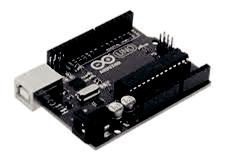
\includegraphics[width=1.65833in,height=1.15833in]{media/image14.jpeg}

La partie précédente a permis de choisir un

correcteur assurant un bon positionnement des

pieds du module SEIS. Cette partie s'intéresse

maintenant à la génération de la consigne de

position à appliquer à chacun de ces pieds via une

carte de commande. \textbf{Figure 14} -- Carte Arduino Uno

On dispose d'une carte Arduino Uno qui peut être programmée dans
différents langages. \textbf{On se} \textbf{limitera à l'utilisation du
langage de programmation Python pour l'étude proposée}.

Le calculateur (la carte Arduino dans notre cas), qui contrôle le
mouvement des trois vérins électriques, génère, pour chaque vérin, un
signal de consigne rapide (vitesse maximale du moteur) ou lent (un
dixième de la vitesse maximale du moteur) en fonction de l'avance de
celui-ci. Dans une première phase, il génère une consigne dite « rapide
» jusqu'à atteindre une distance de 10 mm entre la tige du vérin et le
sol. Le système de commande délivre alors une consigne dite « lente »
afin de limiter les contraintes lors du contact entre chaque vérin et le
sol. Lors de cette deuxième phase (consigne « lente »), un
asservissement en position de chaque vérin permet de maintenir le
châssis du SEIS en position horizontale par rapport au sol.

On note pour la suite de l'étude (\textbf{figure 15}) :

\begin{itemize}
\item
  \textbf{distance} : la variable, de type float, correspondant à la
  distance mesurée entre le sol et le capteur donnée en cm ;
\item
  \textbf{distance\_verin} : la variable, de type float, correspondant à
  la distance entre le capteur et l'extrémité de la tige du vérin donnée
  en cm ;
\item
  \textbf{rapide} et \textbf{lente} : variable globale avec des valeurs
  prédéfinies (correspond aux consignes
\end{itemize}

de la commande du vérin électrique : vitesse rapide, vitesse lente).

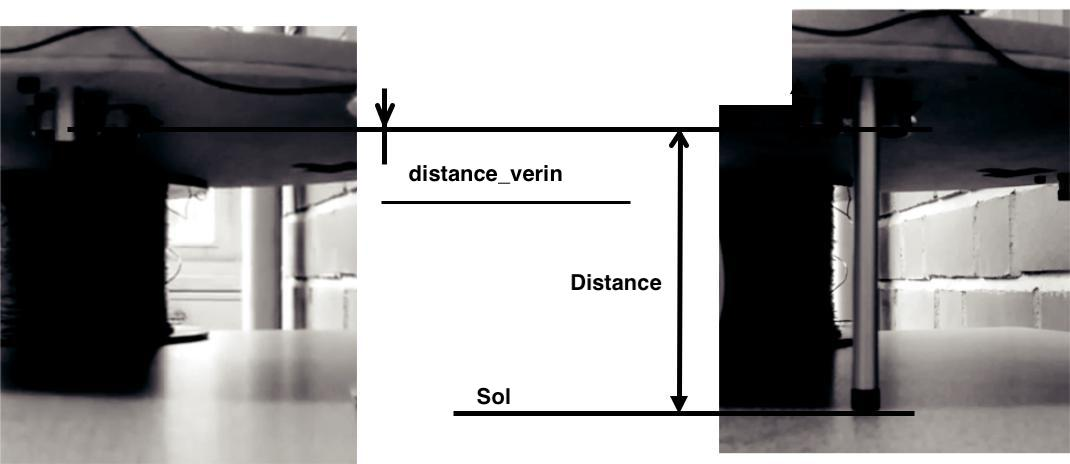
\includegraphics[width=4.95347in,height=2.15000in]{media/image15.jpeg}

capteur

ultrasons
\includegraphics[width=0.24722in,height=0.14861in]{media/image16.jpeg}

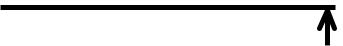
\includegraphics[width=1.58958in,height=0.21111in]{media/image17.jpeg}
distance\_vérin

distance

sol

\textbf{Figure 15} -- Sortie du vérin 1

\textbf{Q26.} Écrire une fonction
\textbf{consigne(distance,distance\_verin)} qui calcule l'écart entre la
tige du vérin et le sol et qui retourne la consigne \textbf{rapide} si
cet écart est supérieur à 10 mm ou

la consigne \textbf{lente} sinon.

\protect\hypertarget{page14}{}{}Le module SEIS est équipé de trois
capteurs de positions, à ultrasons, associés à chaque vérin électrique.
Chaque capteur est constitué d'un émetteur et d'un récepteur à
ultrasons. Le principe de mesure des capteurs à ultrasons utilisés est
donné ci-dessous et illustré sur la \textbf{figure 16}.

Pour déclencher une mesure, il faut présenter une impulsion « High » (5
V) d'au moins 10 µs sur l'entrée « Trig » du capteur (sortie de la carte
Arduino). L'émetteur à ultrasons délivre alors une série de 8 impulsions
ultrasoniques à 40 kHz, puis il attend le signal réfléchi. Lorsque
celui-ci est détecté par le récepteur à ultrasons, le capteur impose un
signal « High » sur la sortie « Echo » (entrée de la

carte Arduino) dont la durée, tc, est proportionnelle à la distance
mesurée. La distance est obtenue en

multipliant la durée du signal tc en seconde par le coefficient constant
17 150 pour obtenir la valeur de la distance en cm.

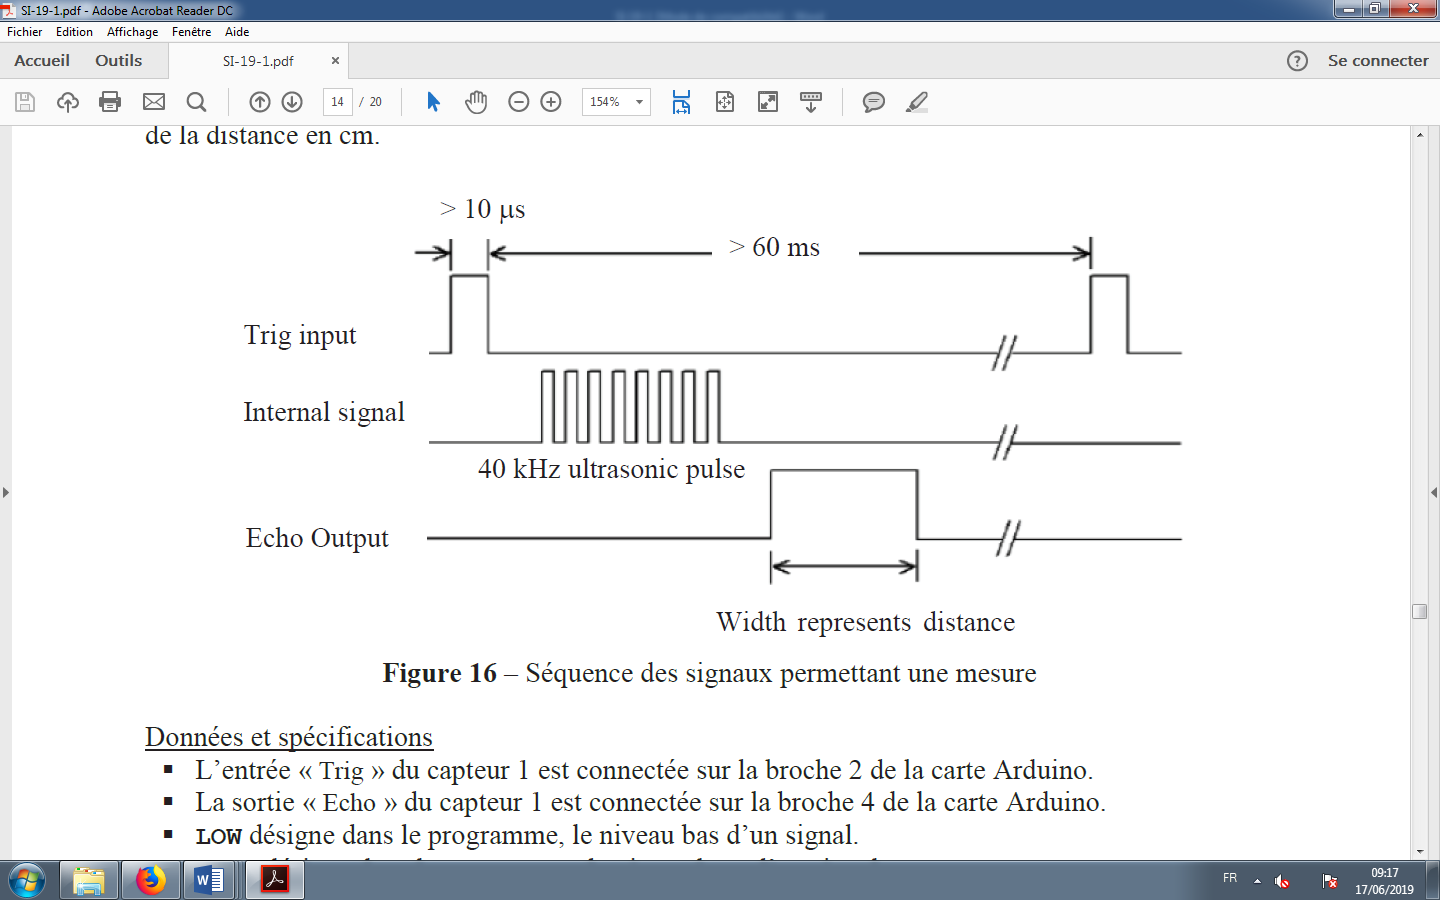
\includegraphics[width=4.56000in,height=2.47917in]{media/image18.png}

\emph{\\
}

\emph{Données et spécifications}

\begin{itemize}
\item
  \begin{quote}
  L'entrée « Trig » du capteur 1 est connectée sur la broche 2 de la
  carte Arduino.
  \end{quote}
\item
  \begin{quote}
  La sortie « Echo » du capteur 1 est connectée sur la broche 4 de la
  carte Arduino.
  \end{quote}
\item
  \begin{quote}
  \textbf{LOW} désigne dans le programme, le niveau bas d'un signal.
  \end{quote}
\item
  \begin{quote}
  \textbf{HIGH} désigne dans le programme, le niveau haut d'un signal.
  \end{quote}
\item
  \begin{quote}
  Les méthodes associées à la gestion des entrées et sorties d'une carte
  Arduino sont données en \textbf{Annexes} (page 16).
  \end{quote}
\item
  \begin{quote}
  Les méthodes associées à la librairie time sont données en
  \textbf{Annexes}.
  \end{quote}
\end{itemize}

\textbf{Q27.} À partir des informations données en \textbf{Annexes},
écrire la fonction \textbf{setup()} qui permet d'initialiser l'entrée et
la sortie de la carte Arduino connectée au capteur 1 et de générer un
signal niveau bas sur la sortie connectée au capteur 1.

On note \textbf{S}, la variable de type entier (int) qui représente le
pin sur lequel on génère une impulsion.

\textbf{Q28.} À partir des informations données en \textbf{Annexes},
écrire la fonction \textbf{impulsion(S)} qui permet

\begin{quote}
de générer une impulsion de niveau haut d'une durée de 20 µs sur la
sortie de la carte Arduino associée à la variable \textbf{S}.
\end{quote}

La fonction \textbf{calcul\_distance(E)} est donnée sur le \textbf{DR4}.
La variable \textbf{E}, de type entier (int), désigne un numéro de pin
de la carte Arduino à identifier à la question \textbf{Q29}.

\protect\hypertarget{page15}{}{}\textbf{Q29.} Commenter le plus
précisément possible sur le \textbf{DR4}, les deux boucles ainsi que les
deux dernières lignes de cette fonction. Que doit-on choisir pour
\textbf{E} si l'on veut utiliser cette fonction pour obtenir la mesure
de distance pour notre capteur 1 ?

\textbf{Q30.} À partir des fonctions \textbf{cacul\_distance(E)} et
\textbf{impulsions(S)}, écrire la fonction \textbf{mesure()} qui
retourne la valeur numérique correspondant à une mesure de position en
cm

\begin{quote}
dans une variable \textbf{mes}. Préciser le type de la variable
\textbf{mes}.
\end{quote}

\textbf{Partie VII - Exploitation de la base de données du système de
mesure (Informatique pour tous)}

\emph{\textbf{Objectif} : analyser et exploiter la base de données des
mesures de la sonde du module SEIS.}

Les différentes mesures obtenues par le module SEIS sont stockées dans
une base de données dont un extrait de la composition des différentes
tables est donné ci-dessous.

\begin{quote}
\textbf{} Table \textbf{Sismique} : elle contient l'ensemble des
mesures de température effectuées par le capteur de température. Le
champ \emph{\textbf{\emph{Mesure}}} correspond au numéro de la mesure,
le champ \emph{\textbf{Date}} correspond à la date de la mesure et le
champ \emph{\textbf{Température}} correspond à la mesure de la
température en °C.

\includegraphics[width=4.23681in,height=0.91389in]{media/image19.png}

\textbf{} Table \textbf{LargeBande} : elle contient l'ensemble des
mesures effectuées par le capteur large bande. Le champ
\emph{\textbf{\emph{Id\_LB}}} correspond au numéro de la mesure, le
champ \emph{\textbf{Date}} correspond à la date de la mesure et les
champs \emph{\textbf{MLBx, MLBy et MLBz}} correspondent aux mesures des
amplitudes des phénomènes sismologiques large bande (0,001 à 10 hertz)
suivant les trois axes x, y et z.

\includegraphics[width=5.92472in,height=0.89571in]{media/image20.png}

\textbf{} Table \textbf{CourteBande} : elle contient l'ensemble des
mesures effectuées par le capteur courte bande. Le champ
\emph{\textbf{\emph{Id\_CB}}} correspond au numéro de la mesure, le
champ \emph{\textbf{Date}} correspond à la date de la mesure et les
champs \emph{\textbf{MCBx, MCBy et MCBz}} correspondent aux mesures des
amplitudes des phénomènes sismologiques courte bande (0,1 à 40 hertz)
suivant les trois axes x, y et z.
\end{quote}

\includegraphics[width=4.47569in,height=1.04236in]{media/image21.png}

\textbf{Q31.} Indiquer le champ qui joue le rôle de clé primaire pour
chaque table de la base de données.

\textbf{Q32.} Donner le résultat de la requête suivante : \textbf{SELECT
Date FROM CourteBande ORDER BY MCBx}.

\protect\hypertarget{page16}{}{}\textbf{Q33.} Donner la requête SQL qui
permet d'obtenir les valeurs de MCBz classées par ordre croissant
suivant la date des évènements et dont les valeurs sont supérieures à
0,2.

\textbf{Q34.} Donner la requête SQL qui permet d'afficher les champs
MLBx, MLBy, MLBz lorsque la température est supérieure à -- 30 °C.

\textbf{Synthèse globale de l'étude}

\textbf{Q35.} Compléter le tableau du \textbf{DR5} en indiquant les
parties de l'étude permettant de valider les exigences indiquées
(validée, non validée, partiellement validée).

\begin{quote}
\textbf{Annexes}
\end{quote}

\emph{Méthodes pour la gestion des entrées et sorties d'une carte
Arduino}

\begin{itemize}
\item
  \begin{quote}
  \textbf{pinMode(pin,mode)}: configure la broche pin choisie en mode
  entrée ou sortie. Le paramètre \textbf{pin} correspond à la valeur de
  la broche de la carte Arduino.
  \end{quote}
\end{itemize}

\begin{quote}
Le paramètre \textbf{mode} peut être choisi entre \textbf{INPUT} pour
associer la broche à une entrée et \textbf{OUTPUT} pour associer la
broche à une sortie.

\emph{Exemple d'utilisation} : l'instruction \textbf{pinMode(4,INPUT)}
permet de configurer la broche 4 comme une entrée.
\end{quote}

\begin{itemize}
\item
  \begin{quote}
  \textbf{digitalWrite(pin,level)} : permet de délivrer une information
  numérique sur la sortie spécifiée.
  \end{quote}
\end{itemize}

\begin{quote}
Le paramètre \textbf{pin} correspond à la valeur de la broche de la
carte Arduino.

Le paramètre \textbf{level} correspond au niveau logique choisi :
\textbf{HIGH} (équivalent du 5 V ou du 1 logique) ou \textbf{LOW}
(équivalent du 0 V ou 0 logique).

\emph{Exemple d'utilisation} : l'instruction
\textbf{digitalWrite(1,LOW)} permet de générer sur la broche 1 un 1
logique.
\end{quote}

\begin{itemize}
\item
  \begin{quote}
  \textbf{digitalRead(pin)} : permet de relever l'information présente
  sur l'entrée spécifiée. Le paramètre \textbf{pin} correspond à la
  valeur de la broche de la carte Arduino.
  \end{quote}
\end{itemize}

\begin{quote}
La méthode retourne l'information sous forme d'une valeur numérique
correspondant à la tension présente sur la broche.

\emph{Exemple d'utilisation} : l'instruction
\textbf{donnée=digitalRead(3)} permet de stocker dans la variable donnée
la valeur de tension lue sur la broche 3.
\end{quote}

\emph{Méthodes de la librairie time}

\begin{itemize}
\item
  \begin{quote}
  \textbf{time.sleep(durée)} : attente d'une durée choisie.
  \end{quote}
\end{itemize}

\begin{quote}
Le paramètre \textbf{durée} correspond à la valeur de l'attente en
seconde.
\end{quote}

\begin{itemize}
\item
  \begin{quote}
  \textbf{time.time()} : délivre l'heure courante.
  \end{quote}
\end{itemize}

\begin{quote}
La méthode retourne l'heure courante exprimée en seconde.
\end{quote}

Documents réponses

\includegraphics[width=6.48194in,height=3.13472in]{media/image22.png}

\includegraphics[width=5.63889in,height=4.52083in]{media/image23.png}

\includegraphics[width=5.83686in,height=4.82418in]{media/image24.png}

\includegraphics[width=4.62009in,height=2.14286in]{media/image25.png}

\includegraphics[width=6.88144in,height=2.99319in]{media/image26.emf}

\end{document}
